\clearpage
\subsection{MSVC: x86 + \olly}

\RU{Попробуем в \olly немного хакнуть программу, и сделать вид что \scanf срабатывает всегда без ошибок}
\EN{Let's try to hack our program in \olly, forcing it to think \scanf working always without error}.

\RU{Когда в \scanf передается адрес локальной перемейнной, изначальное, в данном случае, 
у нас в этой переменной
находится некий мусор, а это}\EN{When address of local variable is passed into \scanf,
initially this variable contain some random garbage, that is} \TT{0x6E494714}\EN{ in case}:

\begin{figure}[H]
\centering
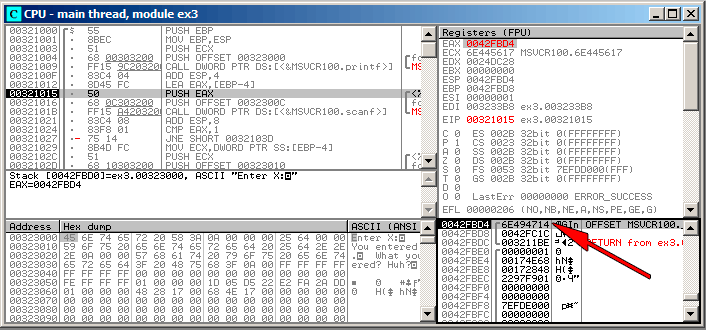
\includegraphics[scale=\FigScale]{patterns/04_scanf/3_checking_retval/olly_1.png}
\caption{\olly: \RU{передача адреса переменной в}\EN{passing variable address into} \scanf}
\label{fig:scanf_ex3_olly_1}
\end{figure}

\clearpage
\RU{Когда}\EN{When} \scanf \RU{запускается, я ввожу в консоли что-то непохожее на число, например}
\EN{is executing, I entered something definitely not a number in the console, like} ``asdasd''.
\scanf \RU{заканчивается с 0 в}\EN{finishing with 0 in} \EAX, \RU{что означает, что произошла ошибка}
\EN{which mean, an error occurred}:

\begin{figure}[H]
\centering
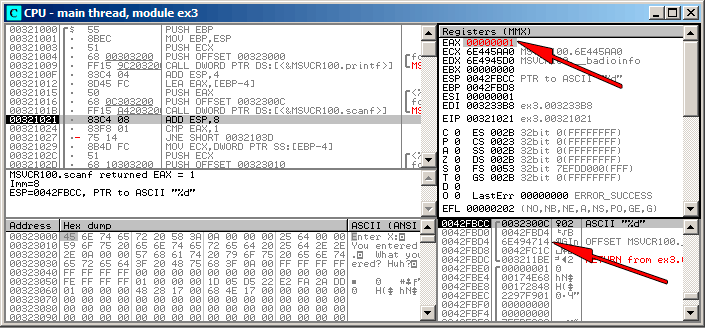
\includegraphics[scale=\FigScale]{patterns/04_scanf/3_checking_retval/olly_2.png}
\caption{\olly: \scanf \RU{закончился с ошибкой}\EN{returning error}}
\label{fig:scanf_ex3_olly_2}
\end{figure}

\RU{Вместе с этим, мы можем посмотреть на локальную переменную в стеке, она не изменилась}
\EN{We can also see to the local variable in the stack and notice that it's not changed}.
\RU{Действительно, ведь что туда записала бы ф-ция \scanf}\EN{Indeed, what \scanf would write there}?
\RU{Она просто ничего не делала кроме возвращения нуля}\EN{It just did nothing except returning zero}.

\RU{А еще попробуем немного ``хакнуть'' нашу программу}\EN{And also let's try to ``hack'' our program}.
\RU{Кликнем правой кнопкой на}\EN{Let's right-click on} \EAX, \RU{там, в числе опций, будет также}
\EN{there will also be} ``Set to 1''\EN{ among other options}.
\RU{Это то что нам нужно}\EN{This is what we need}.

\RU{В \EAX теперь 1, последующая проверка пройдет как надо, и \printf выведет значение переменной
из стека}\EN{1 now in \EAX, so the following check will executed as we need, and \printf will print
value of variable in the stack}.

\RU{Запускаем}\EN{Let's run} (F9) \RU{и видим в консоли следующее}\EN{and we will see this in 
console window}:

\begin{figure}[H]
\centering
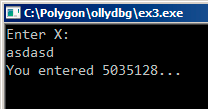
\includegraphics[scale=\FigScale]{patterns/04_scanf/3_checking_retval/olly_3.png}
\caption{\RU{консоль}\EN{console window}}
\end{figure}

\RU{Действительно}\EN{Indeed}, $1850296084$ \RU{это десятичное представление числа в стеке}
\EN{is a decimal representation of the number in stack} (\TT{0x6E494714})!
